\chapter{Classical Runge-Kutta}
In the following, we go back to considering the initial value problem (IVP) on the form
\begin{align}
    \dot{x}(t) &= f(t,x(t),p), & x(t_0) = x_0,
\end{align}
where $x \in \probR ^{n_x}$ and $p \in \probR ^{n_p}$. 

\section{Description of the classical Runge Kutta}
We have previously seen how to use the explicit- or implicit Euler method to solve IVPs. Both of these are first order methods, meaning that their global truncation errors will be directly proportional to the step size of the method, as described in chapter 1. We will now consider a slightly more elaborate method, namely the classical Runge-Kutta method (RK4). 

Again, we wish to determine $x(t+h), \ h>0$ when we know $x(t)$. Via the fundamental theorem of calculus, we have

\begin{align}
    x(t+h) &= x(t) + \int_{t}^{t+h} \dot{x}(t,x(t)) dt.
\end{align}

Notice that our goal now boils down to determining 

\begin{align}
\int_{t}^{t+h} \dot{x}(t,x(t)) dt, \quad h > 0.
\end{align}

If we remember our basic courses in calculus, we remember that there exits many ways to approximate such an integral. The simplest methods are probably the left or right point methods. These correspond to using explicit- or implicit Euler method. The next step is to use the midt point method 

\begin{align}
    x(t+h) &= x(t) + h \cdot \dot{x}\left (t+\frac{h}{2}, x\left (t+\frac{h}{2}\right) \right).
\end{align}

Another is the trapezoidal method

\begin{align}
    x(t+h) &= x(t) + \frac{h}{2} \cdot \dot{x}\left (t, x\left (t\right) \right) + \frac{h}{2} \cdot \dot{x}\left (t+h, x\left (t+h\right) \right).
\end{align}

Notice that this method use a second order Taylor to approximate $x(t)$, which results in integral of an affine function. We could take it one step further and use Simpson's rule, i.e., taking the integral of the approximating quadratic function, then we would get

\begin{align}
    x(t+h) &= x(t) + \frac{h}{6} \left( \dot{x}\left (t, x\left (t\right) \right) + 4 \dot{x}\left (t+ \frac{h}{2}, x\left (t+\frac{h}{2}\right) \right) +\dot{x}\left (t+h, x\left (t+h\right) \right) \right).
\end{align}

Using this approximation, we get what is known as the classical Runge-Kutta method (RK4). The method relies on a non-linear approximation of the original function, as such it approximates it better than first order methods. In fact, RK4 is or order 4\cite{Ascher}. So we have

\begin{align}
    x(t+h) &= x(t) + \frac{h}{6} \left( \dot{x}\left (t, x\left (t\right) \right) + 4 \cdot ...  \right) + \mathcal{O}(h^5).
\end{align}

Now we have the intuition on how RK4 works, however, notice that we do not have all elements on the right hand side. We will therefore dig into how we actually use these methods. In practice, we define for a $s$ stage Runge-Kutta method 

\begin{align}
    T_i &= t_n+c_i \cdot h, \quad i = \{1,2,...,s\}\\
    X_i &= x_n + h \cdot \sum_{j=i}^{s} a_{ij} f(T_j, X_j), \quad i = \{1,2,...,s\},
\end{align}
and
\begin{align}
    t_{n+1} &= t_n + h \\
    x_{n+1} &= x_n + h \cdot \sum_{i=1}^s b_i f(T_i,X_i)
\end{align}
where $x_n=x(t_n)$. We see that the $c_i$'s are used to determine the intermediate time points. The $a_i$'s scale how important each slope estimate is for the individual stages. Finally, the $b_i$'s weights the slopes in relation to the total slope estimate. Often, and for simplicity, we show the parameters in a \textit{butcher tableau}

\begin{align}
    \begin{array}{c|cccc}
         c_1 & & & &   \\
         c_2 & a_{21} & & & \\
         \vdots & \vdots  & \vdots & & \\
         c_s & a_{s1} & a_{s2} & \cdots & \\ \hline 
         x & b_1 & b_2 & \cdots & b_s
    \end{array}
\end{align}
The method is said to be consistent iff we have
\begin{align}
    \sum b_1 = 1.
\end{align}

For the classical Runge-Kutta method, the butcher tableau is given by

\begin{align}
    \begin{array}{c|cccc}
         0   & & & &   \\
         1/2 & 1/2 & & & \\
         1/2 & 0 & 1/2 & & \\
         1   & 0 & 0   & 1 & \\ \hline 
         x   & 1/6 & 1/3 & 1/3 & 1/6.
    \end{array}
\end{align}

The RK4 method is not A- nor L-stable. Figure \ref{fig1:rk4_stability} shows the stability region of RK4 on the test equation. 


\section{Classical Runge Kutta fixed time step implementation}
We now have all theory in place such that we can start using RK4. Listing \ref{lst5:rk4_fixed} shows a Matlab implementation of an explicit Runge-Kutta solver with fixed time step. Notice that to use RK4, we must use the parameters from the butcher tableau. These can be seen in the code below the solver. 

\begin{lstlisting}[language=Matlab,caption=Implementation of explicit Runge-Kutta solver. Parameters corresponding to RK4 given at the end,label=lst5:rk4_fixed]
function [x,t,function_calls,hs] = explicitRungeKutta(f,param,h,t0,T,x0,A,b,c)
    N = ceil((T-t0)/h);
    t = zeros(1,N+1);
    hs = ones(1,N+1);
    hs = h.*hs;
    x = zeros(length(x0),N+1);
    s = length(b);
    k = zeros(length(x0),s)';
    t(1) = t0;
    x(:,1) = x0;
    function_calls = 0;
    
    Ah = h*A;
    bh = h*b;
    ch = h*c;
    
    for i = 2:N+1
       if t(i-1)+h > T
            h = T-t(i-1);
       end
       k = 0*k;
       for j = 1:s
           k(j,:) = f(t(i-1)+ch(j),x(:,i-1)+sum(k.*Ah(j,:)',1)', param);
           function_calls = function_calls +1;
       end
       x(:,i) = x(:,i-1)+sum(k.*bh,1)';
       t(i) = t(i-1)+h;
    end
    x = x';
end

%% RK4 paramters:
A = [0 0 0 0; 0.5 0 0 0; 0 0.5 0 0; 0 0 1 0];
b = [1/6 2/6 2/6 1/6]';
c = [0 1/2 1/2 1]';
p = 4;
\end{lstlisting}


\section{Classical Runge Kutta adaptive time step implementation}
As discussed in previous chapters it can be difficult to select a suitable step size, $h$. When dealing with more advanced problems, particularly stiff problems, we might see that a smaller step size might be required in parts of the solution than others. This problem leads to a desire to construct an algorithm that can change the step size adaptively. The goal is to use as large step size as possible, while maintaining a sufficient accuracy in the individual steps. 

We will again use \textit{step doubling} to estimate the one step errors of the methods, as described in previous chapters. Once again, we are able to define how to select the best step size, $h$. We do so by using the \textit{asymptotic step size controller}. Since RK4 is a 4th order method this means that our step size is given by
\begin{align}
    h_{k+1} &= \left(\frac{\varepsilon}{r_{k+1}} \right )^{1/5} h_k.
\end{align}
Where $r_{k+1}$ is found by
\begin{align}
    r_{k+1} &= \max_{i \in \{1,...,n_x\}} \left \{ \frac{|e_{k+1}|_i}{ \max \{ |\text{abstol}|_i, \ |x_{k+1}|_i \cdot |\text{reltol}|_i \} } \right \}
\end{align}
where $|\text{abstol}|_i$ and $|\text{reltol}|_i$ are the absolute and relative tolerance of $(x_{k+1})_i$ respectively.

Listing \ref{lst5:rk4_adap} shows a Matlab implementation of a general Runge-Kutta solver with error estimation using step doubling and asymptotic step size controller. As before, the specific parameters for RK4 are given below the solver. 

\begin{lstlisting}[language=Matlab,caption=Implementation of explicit Runge-Kutta solver with adaptive time step. Parameters corresponding to RK4 given at the end,label=lst5:rk4_adap]
function [x,t,function_calls,hs] = explicitRungeKuttaDoubling(f,param,h,t0,T,x0,A,b,c,Atol,Rtol,hmin,hmax,eps_tol,p,initial_step_algo)
    N = ceil((T-t0)/hmin);
    s = length(b);
    d = length(x0);
    t = zeros(1,N+1);
    hs = zeros(1,N+1);
    x = zeros(length(x0),N+1);
    k = zeros(d,s)';
    t(1) = t0;
    x(:,1) = x0;
    accept_step = false;
    function_calls = 0;
    
    if initial_step_algo % slide 4b, 9 whic is from p169 Hairer
        [h,function_calls] = initialStepSize(f,param,t0,x0);
    end
    
    i = 2;
    while t(i-1)<=T
       while(~accept_step)
           if t(i-1)+h>T
               h = max(hmin,T-t(i-1));
           end
           
           k = 0*k;
           for j = 1:s
               k(j,:) = f(t(i-1)+h*c(j),x(:,i-1)+sum(h*k.*A(j,:)',1)', param);
               function_calls = function_calls +1;
           end
           oneAhead = x(:,i-1)+sum(h*k.*b,1)';

           hhalf = h/2;
           k = 0*k;
           for j = 1:s
               k(j,:) = f(t(i-1)+hhalf*c(j),x(:,i-1)+sum(hhalf*k.*A(j,:)',1)', param);
               function_calls = function_calls +1;
           end
           halfAhead = x(:,i-1)+sum(hhalf*k.*b,1)';

           k = 0*k;
           for j = 1:s
               k(j,:) = f(t(i-1)+2*hhalf*c(j),halfAhead+sum(hhalf*k.*A(j,:)',1)', param);
               function_calls = function_calls +1;
           end
           halfAhead = halfAhead+sum(hhalf*k.*b,1)';
           
           % Step doubling, see section II.4(s164) in Harier and slide 4c,3
           e = abs(oneAhead-halfAhead);
           r = max(e./max(Atol,abs(halfAhead).*Rtol));
           
           if r<=1
               x(:,i) = halfAhead;
               hs(i-1) = h;
               t(i) = t(i-1)+h;
               accept_step = true;
           else
               accept_step = false;
           end
           h = h*max(hmin,min(hmax,(eps_tol/r)^(1/(1+p)))); % eq 4.13 in Harier
       end
       accept_step = false;
       i = i+1;
    end
    x = x(:,1:i-1)';
    t = t(1:i-1);
    hs = hs(1:i-2);
end

%% RK4 paramters:
A = [0 0 0 0; 0.5 0 0 0; 0 0.5 0 0; 0 0 1 0];
b = [1/6 2/6 2/6 1/6]';
c = [0 1/2 1/2 1]';
p = 4;
\end{lstlisting}


\section{Test on Van der Pol problem and comparison with Matlab ODE solvers}
Now that we have made an implementation of the classical Runge Kutta method with both fixed and adaptive step size we want to compare these. To do so we look at the Van der Pol problem given by
\begin{align}
    \Ddot{x}(t) &= \mu (1-x(t)^2) \dot{x}(t) - x(t).
\end{align}
To solve the problem we must first re-write the problem as a system of first order differential equations. Luckily this is done easily and given by
\begin{align}
    \dot{x}_1(t) &= x_2(t) \\
    \dot{x}_2(t) &= \mu(1-x_1(t)^2) x_2(t) - x_1(t).
\end{align}

We will now test the classical Runge Kutta method on the Van der Pol problem with $\mu = 3$ and $\mu = 20$. 

\subsection{Van der Pol, $\mu = 3$}
The Van der Pol problem with $\mu = 3$ is a relatively straight forward non-stiff problem. There is no formal definition of when a problem is \textit{stiff}---only that whenever a problem change dynamics "very quickly" it is said to be. 

Figure \ref{fig5:fixed_mu3} shows the numerical solution to the Van der Pol problem with $\mu = 3$ for RK4 with $h \in \{0.1, 0.01, 0.001\}$, ODE45 and ODE15s. Notice that there is no visible difference between the solution obtained by ODE45 and ODE15s. Notice also that for already for $h=0.1$ there is almost no difference between RK4 and ODE45/ODE15s. If we look very closely, we can see some small local deviation in the line, however, they are actually not because the method is wrong, the distance between the estimated points are just so big, that we can see the straight line Matlab draws between them. It seems that this problem is an easy task for the RK4 method, even with relatively large step sizes.

\begin{figure}[H]
    \centering
    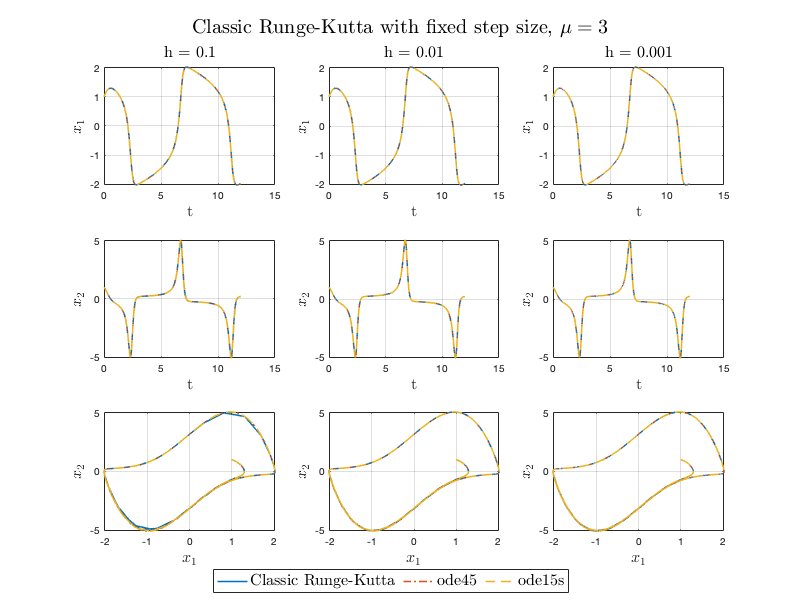
\includegraphics[width=\textwidth]{graphics/opg5/mu3_fixed.png}
    \caption{Solution to Van der Pol with $\mu = 3$ using fixed step sizes}
    \label{fig5:fixed_mu3}
\end{figure}

Table \ref{tab5:mu3_fixed} shows that CPU time and number of function evaluations when solving the Van der Pol problem with $\mu = 3$ using different time steps and Matlab ODE solvers. Notice that with $h=0.1$ the RK4 uses the fewest function calls of any of the methods. Even so, the ODE45 is still as fast---which might be a bit surprising. The issue here is that when we call our own function, they are made in Matlab. Therefore there will be some overhead on the run time. This has been minimized on the build in functions, which makes the Matlab function very difficult to beat when comparing run-times. 

Notice that ODE45 seems to outperform ODE15s. This is a good indication that the problem is not particular stiff, i.e., it is not worth while to use an implicit method that comes with additional computational cost. 

\begin{table}[H]
    \centering
    \caption{CPU time and function evaluations of classical Runge Kutta with fixed time step and Matlab ODE solvers}
    \begin{tabular}{|c||c|c|c|c|c|c|} \hline
         \textbf{Method}    & $h=0.1$&   $h=0.01$ & $h=0.001$ & ODE45 & ODE15s     \\ \hline \hline 
         \textbf{Time}      & 0.0042 &   0.0196 &   0.2029 &  0.0046 & 0.0175   \\ \hline
         \textbf{Fun evals} & 480     &   4800   &    48000 & 1069 & 926  \\ \hline
    \end{tabular}
    \label{tab5:mu3_fixed}
\end{table}



Figure \ref{fig5:adap_mu3} shows the numerical solution to the Van der Pol problem with $\mu = 3$ for the classical Runge Kutta with adaptive time steps and $AbsTol=RelTol \in \{10^{-2}, 10^{-4}, 10^{-6}\}$, ODE45 and ODE15s. Notice also that for $Tol = 10^{-2}$ we again see some difference in the plots. Once again, it is simply because at the tolerance, the RK4 take such large time steps, that we can see the straight lines by Matlab. This is especially visible in the "corner" of the solution curve.

\begin{figure}[H]
    \centering
    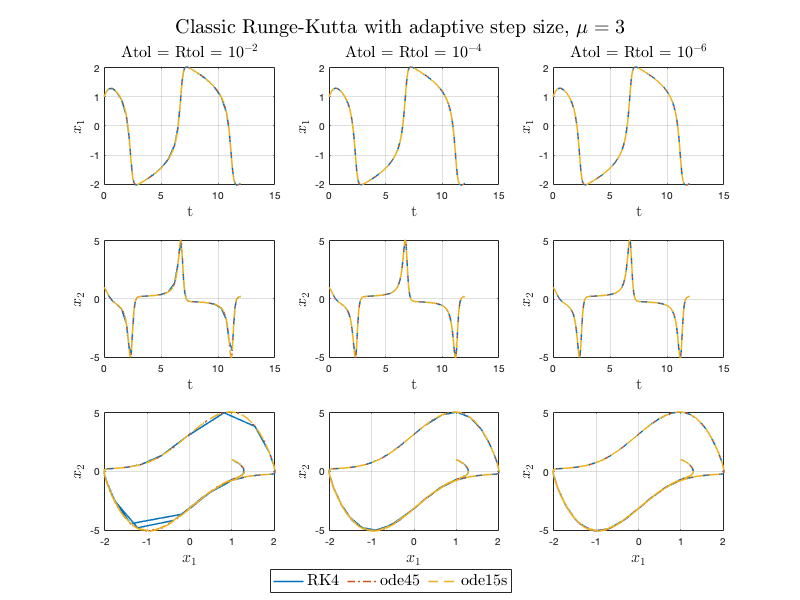
\includegraphics[width=\textwidth]{graphics/opg5/mu3_adap.png}
    \caption{Solution to Van der Pol with $\mu = 3$ using adaptive step sizes}
    \label{fig5:adap_mu3}
\end{figure}

Table \ref{tab5:mu3_adap} shows the CPU time and number of function evaluations when solving the Van der Pol problem with $\mu = 3$ using different tolerances and Matlab ODE solvers. Notice that with $Tol = 10^{-2}$ the RK4 is relatively fast (slower than ODE45 but as fast as ODE15s). Generally, it is very hard to tell the solutions curves apart just by looking at them. Even for the lowest tolerance, we get quite good results. What is interesting is the CPU time usage and number of function evaluations used at the different tolerances. For both explicit- and implicit Euler, we saw that the CPU time and function evaluations increased dramatically when we required higher accuracy, now this increase is not as pronounced. This demonstrates the power of higher order methods quite well.

One of the reasons why ODE45 is able to outperform the RK4 with adaptive step size is because it used an embedded error estimate, i.e., not step doubling. Using an embedded error estimate is a more efficient way of estimating the errors and hence the algorithm is faster.

\begin{table}[H]
    \centering
    \caption{CPU time and function evaluations of RK4 with adaptive time step and Matlab ODE solvers}
    \begin{tabular}{|c||c|c|c|c|c|c|} \hline
         \textbf{Method}    & $Tol = 10^{-2}$&   $Tol = 10^{-4}$ & $Tol = 10^{-6}$ & ODE45 & ODE15s     \\ \hline \hline 
         \textbf{Time}      & 0.0209 &   0.0622 &    0.0577 & 0.0046 & 0.0175   \\ \hline
         \textbf{Fun evals} & 758   &     1562   &     3374 & 1069 & 926  \\ \hline
    \end{tabular}
    \label{tab5:mu3_adap}
\end{table}

Figure \ref{fig5:adap_mu3_h} shows the used step sizes for the different tolerances. The red crosses mark whenever the step size controller failed to set the step size correctly, i.e., whenever the estimated (using step doubling) error was larger than the allowed maximum. Notice that the behaviour of all three tolerances are quite similar. Also notice that the step sizes does not vary nearly as much for the individual tolerances as previously seen (for explicit- and implicit Euler). Additionally, if we look at the difference in step sizes for the different tolerances, we see that in order to decrease the tolerance by a factor $10^4$, we only need to decrease the step size by a factor $10^1$. This is the true power of higher order methods! And shows that the RK4 is indeed of order 4. 

\begin{figure}[H]
    \centering
    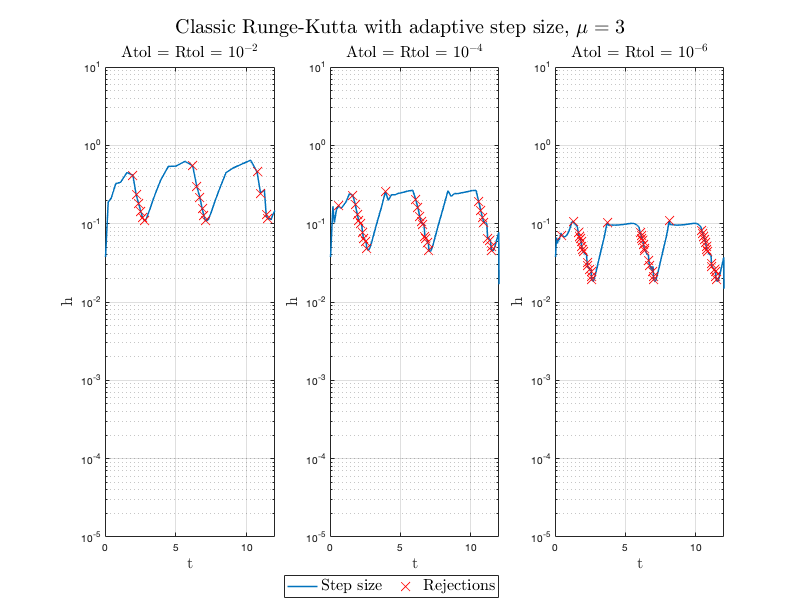
\includegraphics[width=\textwidth]{graphics/opg5/mu3_h.png}
    \caption{Step sizes when solving the Van der Pol with $\mu = 3$ at different tolerances}
    \label{fig5:adap_mu3_h}
\end{figure}

\subsection{Van der Pol, $\mu = 20$}
The Van der Pol problem with $\mu = 20$ is a more complicated problem. The dynamics of the problem is largely defined by the $\mu$ parameter. In particular, the problem becomes more stiff when $\mu$ is increased.

Figure \ref{fig5:fixed_mu20} shows the numerical solution to the Van der Pol problem with $\mu = 20$ for RK4 with $h \in \{0.1, 0.01, 0.001\}$, ODE45 and ODE15s. Notice that there is no visible difference between the solution obtained by ODE45 and ODE15s. For $h=0.1$ the solution once again diverged (as the explicit Euler did). This demonstrated the unfortunate weak property of explicit methods in general. Explicit methods generally have much worse convergence properties compared to implicit methods. In chapter 1 we also showed that RK4 is neither A- nor L-stable, and has a region of stability fairly similar to that of the explicit Euler method. However, when RK4 is within its region of stability, the results are quite good. For both $h=0.01$ and $h=0.001$ there are no visible difference between RK4 and ODE45/ODE15s. 

\begin{figure}[H]
    \centering
    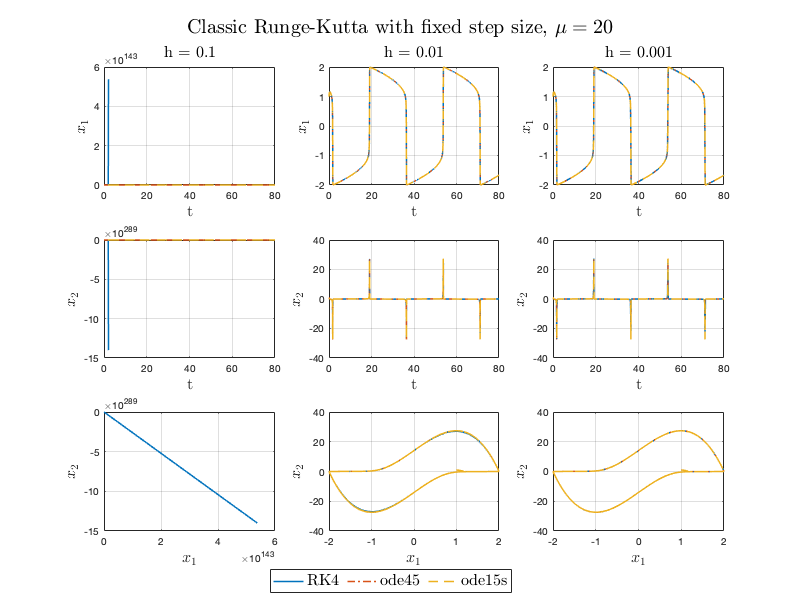
\includegraphics[width=\textwidth]{graphics/opg5/mu20_fixed.png}
    \caption{Solution to Van der Pol with $\mu = 20$ using fixed step sizes}
    \label{fig5:fixed_mu20}
\end{figure}

Table \ref{tab5:mu20_fixed} shows that CPU time and number of function evaluations when solving the Van der Pol problem with $\mu = 20$ using different time steps and Matlab ODE solvers. Notice that with $h=0.1$ the RK4 is faster than any of the other methods, however, as seen above the results are also completely wrong. At a time step of $h=0.01$ RK4 is already slower than ODE45/ODE15s and use many more function calls. At this point there is also no visible difference the results. 

Notice that ODE45 does not outperform ODE15s anymore. This is a good indication that the problem is stiff, i.e., it is worth while to use an implicit method that even when it comes with additional computational cost. The implicit method is also able to use far less function evaluations than the DoPri54. 

\begin{table}[H]
    \centering
    \caption{CPU time and function evaluations of RK4 with fixed time step and Matlab ODE solvers}
    \begin{tabular}{|c||c|c|c|c|c|c|} \hline
         \textbf{Method}    & $h=0.1$&   $h=0.01$ & $h=0.001$ & ODE45 & ODE15s     \\ \hline \hline 
         \textbf{Time}      & 0.0179   & 0.1187  &  1.0235 & 0.0370 & 0.0504   \\ \hline
         \textbf{Fun evals} & 3200    &   32000   &   320000 & 8461 & 926  \\ \hline
    \end{tabular}
    \label{tab5:mu20_fixed}
\end{table}



Figure \ref{fig5:adap_mu20} shows the numerical solution to the Van der Pol problem with $\mu = 20$ for the classical Runge Kutta method with adaptive time steps and $AbsTol=RelTol \in \{10^{-2}, 10^{-4}, 10^{-6}\}$, ODE45 and ODE15s. Notice also that for $Tol = 10^{-2}$ the only difference visible is again due to the relatively large steps that the algorithm takes in the "non-stiff" area. Otherwise, all tolerances seem to follow the ODE45/ODE15s solutions very well.

\begin{figure}[H]
    \centering
    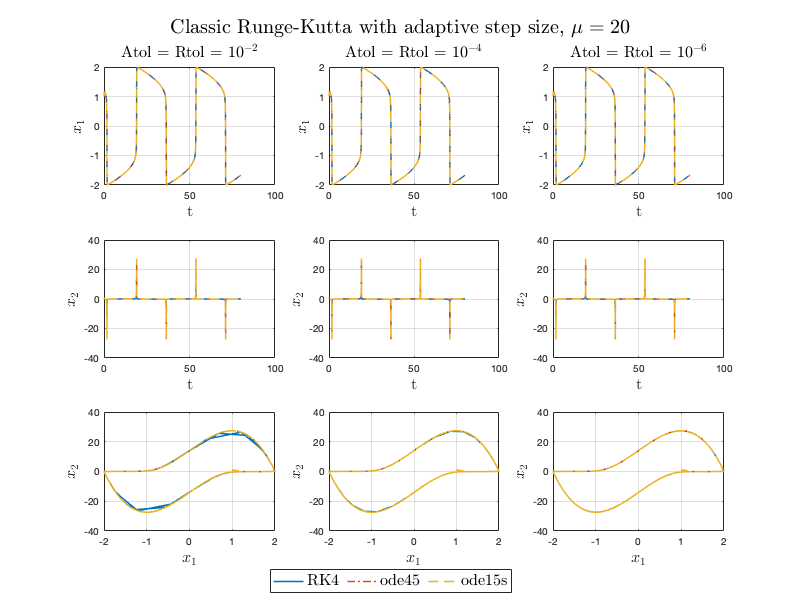
\includegraphics[width=\textwidth]{graphics/opg5/mu20_adap.png}
    \caption{Solution to Van der Pol with $\mu = 20$ using adaptive step sizes}
    \label{fig5:adap_mu20}
\end{figure}

Table \ref{tab5:mu20_adap} shows that CPU time and number of function evaluations when solving the Van der Pol problem with $\mu = 20$ using different tolerances and Matlab ODE solvers. Notice that with $Tol = 10^{-2}$ the RK4 is very similar in speed and number of function calls to ODE45 (and faster then ODE15s). Once again notice that 100 times the accuracy does not require 100 times the CPU time or 100 times the function calls. This is because RK4 is a 4th order method, i.e., the accuracy increase much faster than linear. 

\begin{table}[H]
    \centering
    \caption{CPU time and function evaluations of RK4 with adaptive time step and Matlab ODE solvers}
    \begin{tabular}{|c||c|c|c|c|c|c|} \hline
         \textbf{Method}    & $Tol = 10^{-2}$&   $Tol = 10^{-4}$ & $Tol = 10^{-6}$ & ODE45 & ODE15s     \\ \hline \hline 
         \textbf{Time}      & 0.0365  &  0.2100  &  0.2309 & 0.0386 & 0.0612   \\ \hline
         \textbf{Fun evals} &  9194    &   11306   &    18626 & 8461 & 2944  \\ \hline
    \end{tabular}
    \label{tab5:mu20_adap}
\end{table}

Figure \ref{fig5:adap_mu20_h} shows the used step sizes for the different tolerances. The red crosses mark whenever the step size controller failed to set the step size correctly, i.e., whenever the estimated (using step doubling) error was larger than the allowed maximum. Notice that the behaviour of all three tolerances are quite similar. Also notice that the step sizes does not vary nearly as much for the individual tolerances as previously seen (for explicit- and implicit Euler). Additionally, if we look at the difference in step sizes for the different tolerances, we see that in order to decrease the tolerance by a factor $10^4$, we only need to decrease the step size by a factor $10^1$. This is the true power of higher order methods! And shows that the RK4 is indeed of order 4. 

Finally, notice that the estimated step sizes are quite often rejected, i.e., the step size controller underestimated the need for more accuracy. Judging by the number of rejection for this fairly stiff problem, it might be worthwhile to consider other controller, e.g. a PID controller instead of the asymptotic step size controller we are currently using. 

\begin{figure}[H]
    \centering
    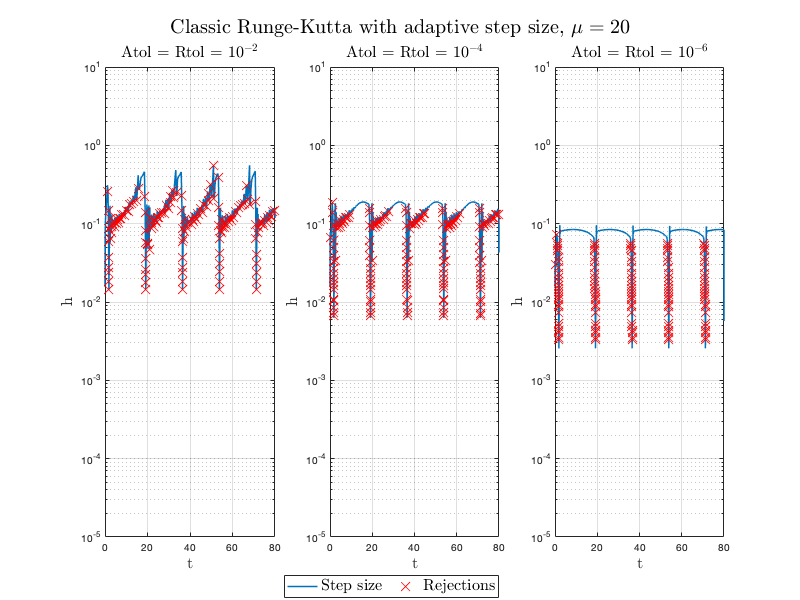
\includegraphics[width=\textwidth]{graphics/opg5/mu20_h.png}
    \caption{Step sizes when solving the Van der Pol with $\mu = 20$ at different tolerances}
    \label{fig5:adap_mu20_h}
\end{figure}





